\documentclass[../../main/main.tex]{subfiles}
\graphicspath{{./figures/}}

\dominitoc
\faketableofcontents

% \renewcommand{\mtcSfont}{\small\bfseries}
% \renewcommand{\mtcSSfont}{\footnotesize}
\mtcsettitle{minitoc}{}
\mtcsetrules{*}{off}

\makeatletter
\renewcommand{\@chapapp}{Optique -- chapitre}
\renewcommand{\chaplett}{O}
\makeatother

% \toggletrue{student}
% \toggletrue{corrige}
% \renewcommand{\mycol}{black}
% \renewcommand{\mycol}{gray}

\hfuzz=5.002pt

\begin{document}
\setcounter{chapter}{1}

\settype{book}
\settype{prof}
\settype{stud}

\chapter{Base de l'optique g\'eom\'etrique}

\vspace*{\fill}

\begin{tcn}(appl)<ctc>"somm"'t'{Sommaire}
	\let\item\olditem
	\vspace{-15pt}
	\minitoc
	\vspace{-25pt}
\end{tcn}

\begin{tcn}[sidebyside](appl)<ctb>"how"'t'{Capacités exigibles}
	\begin{itemize}[label=\rcheck]
		\item Définir le modèle de l'optique géométrique et indiquer ses limites.
		\item Énoncer les lois de \textsc{Snell-Descartes}.
		\item Définir une convention d'orientation des angles et travailler avec
		      des angles orientés.
		\item Savoir que l'interprétation par le cerveau de la trajectoire des
		      rayons lumineux joue un rôle dans certains phénomènes optiques.
		\item Connaître le vocabulaire des systèmes optiques.
	\end{itemize}
	\tcblower
	\begin{itemize}[label=\rcheck]
		\item Énoncer les conditions de l'approximation de \textsc{Gauss} et ses
		      conséquences.
		\item Établir les conditions de réflexion totale.
		\item Utiliser les lois de \textsc{Snell-Descartes}.
		\item Identifier la nature réelle ou virtuelle d'un objet ou d'une image.
		\item Dessiner des rayons lumineux à travers un système optique de manière
		      cohérente avec les indices optiques.
		\item Établir les expressions du cône d'acceptance et de la dispersion
		      intermodale d'une fibre à saut d'indice.
	\end{itemize}
\end{tcn}

\vspace*{\fill}
\newpage
\vspace*{\fill}

%\vspace{-15pt}
\begin{tcn}[sidebyside, fontupper=\small, fontlower=\small](appl)<ctb>"chek"'t'{L'essentiel}
	\begin{tcn}(defi)<ctc>'t'{Définitions}
		\tcblistof[\paragraph*]{defi}{\hspace*{4.8pt}}
	\end{tcn}
	% \begin{tcn}(rapp)<ctc>'t'{Rappels}
	% 	\tcblistof[\paragraph*]{rapp}{\hspace*{4.8pt}}
	% \end{tcn}
	% \begin{tcn}(prop)<ctc>'t'{Propriétés}
	% 	\tcblistof[\paragraph*]{prop}{\hspace*{4.8pt}}
	% 	\tcblistof[\paragraph*]{loi}{\hspace*{4.8pt}}
	% 	% \tcblistof[\paragraph*]{theo}{\hspace*{4.8pt}}
	% \end{tcn}
	% \begin{tcn}(coro)<ctc>'t'{Corollaires}
	%   \tcblistof[\paragraph*]{coro}{\hspace*{4.8pt}}
	% \end{tcn}
	% \begin{tcn}(demo)<ctc>'t'{Démonstrations}
	% 	\tcblistof[\paragraph*]{demo}{\hspace*{4.8pt}}
	% 	\tcblistof[\paragraph*]{prev}{\hspace*{4.8pt}}
	% \end{tcn}
	% \begin{tcn}(inte)<ctc>'t'{Interprétations}
	% 	\tcblistof[\paragraph*]{inte}{\hspace*{4.8pt}}
	% \end{tcn}
	% \begin{tcn}(impl)<ctc>'t'{Implications}
	% 	\tcblistof[\paragraph*]{impl}{\hspace*{4.8pt}}
	% \end{tcn}
	% \begin{tcn}(tool)<ctc>'t'{Outils}
	% 	\tcblistof[\paragraph*]{tool}{\hspace*{4.8pt}}
	% \end{tcn}
	\begin{tcn}(nota)<ctc>'t'{Notations}
		\tcblistof[\paragraph*]{nota}{\hspace*{4.8pt}}
	\end{tcn}
	% \begin{tcn}(appl)<ctc>'t'{Applications}
	% 	\tcblistof[\paragraph*]{appl}{\hspace*{4.8pt}}
	% \end{tcn}
	% \begin{tcn}(rema)<ctc>'t'{Remarques}
	%   \tcblistof[\paragraph*]{rema}{\hspace*{4.8pt}}
	% \end{tcn}
	% \begin{tcn}(exem)<ctc>'t'{Exemples}
	%   \tcblistof[\paragraph*]{exem}{\hspace*{4.8pt}}
	% \end{tcn}
	% \begin{tcn}*(ror)<ctc>"hart"'t'{Points importants}
	%   \tcblistof[\paragraph*]{ror}{\hspace*{4.8pt}}
	% \end{tcn}
	% \begin{tcn}(impo)<ctc>'t'{Erreurs communes}
	%   \tcblistof[\paragraph*]{impo}{\hspace*{4.8pt}}
	% \end{tcn}
	\tcblower
	% \begin{tcn}(defi)<ctc>'t'{Définitions}
	%   \tcblistof[\paragraph*]{defi}{\hspace*{4.8pt}}
	% \end{tcn}
	% \begin{tcn}(rapp)<ctc>'t'{Rappels}
	%   \tcblistof[\paragraph*]{rapp}{\hspace*{4.8pt}}
	% \end{tcn}
	\begin{tcn}(prop)<ctc>'t'{Propriétés}
		\tcblistof[\paragraph*]{prop}{\hspace*{4.8pt}}
		% \tcblistof[\paragraph*]{loi}{\hspace*{4.8pt}}
		% \tcblistof[\paragraph*]{theo}{\hspace*{4.8pt}}
	\end{tcn}
	% \begin{tcn}(coro)<ctc>'t'{Corollaires}
	%   \tcblistof[\paragraph*]{coro}{\hspace*{4.8pt}}
	% \end{tcn}
	\begin{tcn}(demo)<ctc>'t'{Démonstrations}
		\tcblistof[\paragraph*]{demo}{\hspace*{4.8pt}}
		% \tcblistof[\paragraph*]{prev}{\hspace*{4.8pt}}
	\end{tcn}
	% \begin{tcn}(inte)<ctc>'t'{Interprétations}
	% 	\tcblistof[\paragraph*]{inte}{\hspace*{4.8pt}}
	% \end{tcn}
	\begin{tcn}(impl)<ctc>'t'{Implications}
		\tcblistof[\paragraph*]{impl}{\hspace*{4.8pt}}
	\end{tcn}
	% \begin{tcn}(tool)<ctc>'t'{Outils}
	%   \tcblistof[\paragraph*]{tool}{\hspace*{4.8pt}}
	% \end{tcn}
	% \begin{tcn}(nota)<ctc>'t'{Notations}
	%   \tcblistof[\paragraph*]{nota}{\hspace*{4.8pt}}
	% \end{tcn}
	% \begin{tcn}(odgr)<ctc>'t'{Ordres de grandeur}
	% 	\tcblistof[\paragraph*]{odgr}{\hspace*{4.8pt}}
	% \end{tcn}
	% \begin{tcn}(appl)<ctc>'t'{Applications}
	% 	\tcblistof[\paragraph*]{appl}{\hspace*{4.8pt}}
	% \end{tcn}
	% \begin{tcn}(rema)<ctc>'t'{Remarques}
	%   \tcblistof[\paragraph*]{rema}{\hspace*{4.8pt}}
	% \end{tcn}
	% \begin{tcn}(exem)<ctc>'t'{Exemples}
	% 	\tcblistof[\paragraph*]{exem}{\hspace*{4.8pt}}
	% \end{tcn}
	% \begin{tcn}*(ror)<ctc>"hart"'t'{Points importants}
	% 	\tcblistof[\paragraph*]{ror}{\hspace*{4.8pt}}
	% \end{tcn}
	\begin{tcn}(impo)<ctc>'t'{Erreurs communes}
		\tcblistof[\paragraph*]{impo}{\hspace*{4.8pt}}
	\end{tcn}
\end{tcn}

\vspace*{\fill}

\newpage

\section{Propriétés générales}
\subsection{Optique non géométrique~: diffraction de la lumière}
\label{ssec:optdiff}
\subsubsection{Principe}

\noindent
\begin{minipage}[t]{.48\linewidth}
	La nature ondulatoire de la lumière apparaît clairement lors des expériences de
	diffraction~: dans certains cas, la restriction d'un faisceau lumineux (par
	exemple un laser) par une fente, donne sur un écran placé loin derrière, un
	étalement de la lumière \textbf{plus large} que la largeur de la fente.
	\smallbreak
	Ce phénomène survient quand l'extension spatiale d'une onde est limitée~; cela
	arrive également avec les vagues dans l'eau. En effet, pour des valeurs de
	largeur de fente $a \gg \lambda$, il n'y a bien qu'une coupure du faisceau. En
	revanche, quand $a \approx \lambda$, ce phénomène survient. On observe même que
	plus $a$ est petit, plus la lumière s'étale sur l'écran.
\end{minipage}
\hfill
\begin{minipage}[t]{.48\linewidth}
	~
	\vspace*{-30pt}
	\begin{center}
		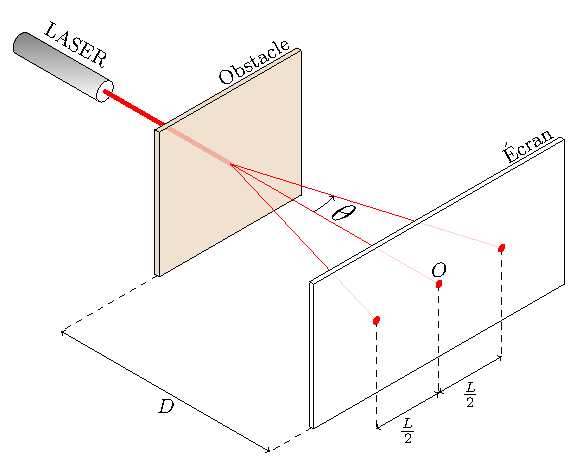
\includegraphics[width=.8\linewidth]{diffraction}
		\captionof{figure}{Diffraction de \textsc{Fraunhofer} d'un faisceau laser par
			une fente fine.}
		\label{fig:diff_las}
	\end{center}
\end{minipage}

\subsubsection{Loi de la diffraction}

\begin{tcb*}[label=prop:loidiff](prop){Diffraction par une fente simple}
	Un faisceau monochromatique de longueur d'onde $\lambda$ dans le vide,
	limité spatialement par une fente de largeur $a \approx \lambda$, forme à
	grande distance sur un écran des tâches lumineuses dont le demi angle
	d'ouverture $\theta$ de la tâche centrale vérifie
	\psw{%
		\[
			\boxed{\sin(\theta) = \frac{\lambda}{a}}
		\]
	}%
	\vspace*{-10pt}
\end{tcb*}

\subsection{Approximation de l'optique géométrique}

\subsubsection{Définition}

\begin{tcb*}[label=def:optgeo,
		list entry={\lte Approxima$^\circ$ de l'optiq.\ géométrique}
	](defi){Approximation de l'optique géométrique}
	\psw{%
		L'approximation de l'optique géométrique consiste à \textbf{négliger tout
			phénomène de diffraction} (et d'interférence, cf.\ chapitres plus avancés)
		pour ignorer le comportement ondulatoire de la lumière. Dans cette approche,
		la lumière est équivalente à un flux de particules \textit{indépendantes},
		sans interaction globale (propriété d'une onde)~: c'est le modèle
		\textbf{corpusculaire}.
	}%
\end{tcb*}

\subsubsection{Notion de rayon lumineux}

Dans le cadre de l'optique géométrique, on décrit donc la lumière par la
trajectoire des photons.

\begin{tcb*}[cnt, bld, label=def:rl](defi){Rayon et faisceau lumineux}
	\psw{%
		Un rayon lumineux est une courbe orientée donnant la direction et le sens de
		propagation d'une onde lumineuse. Un faisceau est un ensemble de rayons.
	}%
\end{tcb*}
\begin{tcb}(rema)<lftt>{}
	C'est un outil théorique~: il est impossible d'isoler un rayon lumineux
	en pratique à cause de la diffraction.
\end{tcb}

\subsubsection{Propriétés d'un rayon lumineux}

\begin{tcb*}[label=prop:rl](prop){Propriétés d'un rayon lumineux}
	\begin{enumerate}
		\item[b]{Propagation rectiligne}: \psw{%
			Dans un milieu TLHI, la lumière se propage en ligne droite.
		}%
		\item[b]{Indépendance des rayons}: \psw{%
			Les rayons lumineux n'interfèrent pas entre eux. Notamment, un rayon ne
			peut pas en dévier un autre.
		}%
		\item[b]{Retour inverse}: \psw{%
			Dans un milieu TLI, homogène ou non, si une source en A éclaire B, alors
			une source placée en B éclaire A.
		}%
		\begin{center}
			% TODO: Reprendre schéma Schweitzer
			\sswitch{
				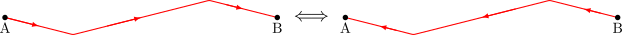
\includegraphics[width=\linewidth, draft=true]{retour_inv}
			}{
				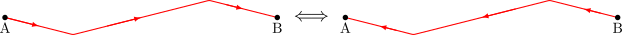
\includegraphics[width=\linewidth]{retour_inv}
			}%
			\captionsetup{justification=centering}
			\captionof{figure}{Schématisation du principe de retour inverse de la
				lumière.}
		\end{center}
	\end{enumerate}
\end{tcb*}

\subsubsection{Limites du modèle}

\begin{itemize}[label=$\diamond$, leftmargin=10pt]
	\item[b]{Diffraction}~: voir \ref{ssec:optdiff}~;
	\item[b]{Phénomènes ondulatoires}~: le modèle de rayon n'explique pas les
	interférences (voir plus tard dans l'année)~;
	\item[b]{Polarisation}~: en tant qu'oscillations des champs électrique et
	magnétique $\vv{E}$ et $\vv{B}$, elle est dotée d'une orientation et est à
	l'origine de nombreux phénomènes optiques (cinéma 3D par exemple)~;
	\item[b]{Inhomogénéité}~: dans un milieu inhomogène, la lumière ne se propage
	pas en ligne droite et donne lieux aux mirages.
\end{itemize}

\begin{figure}[htbp]
	\centering
	% TODO: Reprendre schéma Schweitzer
	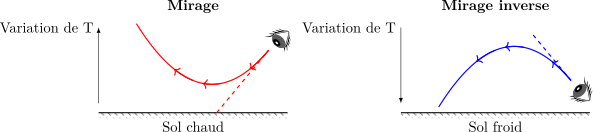
\includegraphics[width=\linewidth]{mirages}
	\caption{Représentation d'un mirage chaud, où la lumière vient du ciel en
		regardant le sol, et d'un mirage froid, où c'est l'inverse.}
	\label{fig:mirages}
\end{figure}

\section{Lois de Snell-Descartes}
\subsection{Changement de milieu}

\begin{tcb*}[label=def:dioptre, sidebyside, righthand ratio=.4](defi){Dioptre}
	\psw{%
		On appelle «~dioptre~» la surface de séparation entre deux
		milieux transparents d'indices optiques différents.
	}%
	\tcblower
	\begin{center}
		\sswitch{
			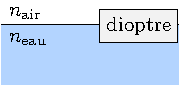
\includegraphics[width=4cm, draft=true]{dioptre}
			\label{fig:dioptre}
		}{
			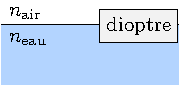
\includegraphics[width=4cm]{dioptre}
			\label{fig:dioptre}
		}%
		\captionof{figure}{Exemple de dioptre.}
	\end{center}
\end{tcb*}
% \sde[right, label=prop:r_dioptre](prop){Réflexion, réfraction}{
% 	Au niveau d'un dioptre, un rayon lumineux incident donne
% 	naissance à un rayon réfracté (traversant le dioptre) et à un
% 	rayon réfléchi.
% }{
% 	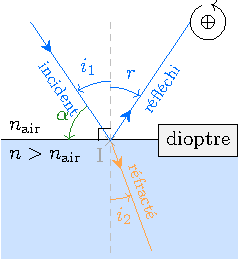
\includegraphics[width=3cm]{dioptre_rl}
% 	\captionof{figure}{Rayons incidents, réfléchis et réfractés
% 		sur un dioptre.}
% 	\label{fig:dioptre_rl}
% }%

\begin{tcb*}[label=prop:r_dioptre, sidebyside,
		righthand ratio=.45](prop){Réflexion, réfraction}
	Au niveau d'un dioptre, un rayon lumineux \textbf{incident} donne
	naissance à~:
	\begin{itemize}[label=$\diamond$, leftmargin=10pt]
		\item un rayon réfracté (traversant le dioptre)~;
		\item un rayon réfléchi.
	\end{itemize}
	\tcblower
	\begin{center}
		\sswitch{
			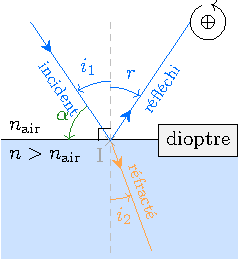
\includegraphics[width=5cm, draft=true]{dioptre_rl}
			\label{fig:dioptre_rl}
		}{
			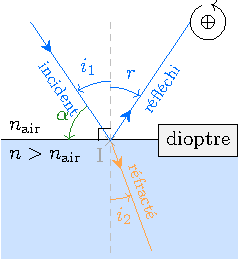
\includegraphics[width=5cm]{dioptre_rl}
			\label{fig:dioptre_rl}
		}%

		\captionof{figure}{Rayons incidents, réfléchis et réfractés
			sur un dioptre.}
	\end{center}
\end{tcb*}
\begin{tcb*}[label=nota:descartes](nota)<lftt>{Vocabulaire général}
	\begin{itemize}[label=$\diamond$, leftmargin=10pt]
		\item[b]{Point d'incidence} I~: \psw{%
			intersection du rayon incident avec le dioptre~;
		}%
		\item[b]{Plan d'incidence}~: \psw{%
			contient le rayon incident et la normale au dioptre en I~;
		}%
		\item[b]{Angle d'incidence} $i_1$~: \psw{%
			angle entre la normale et le rayon incident~;
		}%
		\item[b]{Angle de réflexion} $r$~: \psw{%
			angle entre la normale et le rayon réfléchi~;
		}%
		\item[b]{Angle de réfraction} $i_2$~: \psw{%
			angle entre la normale et le rayon réfracté.
		}%
	\end{itemize}
\end{tcb*}
\begin{tcb*}*[label=ror:normale, fontupper=\Huge](impo)"bomb"{Calcul des angles}
	Les angles se calculent entre le rayon et la \textbf{normale} au dioptre. Le
	sens de comptage doit être indiqué sur la figure.
\end{tcb*}

\subsection{Lois de Snell-Descartes}

\begin{tcb*}[label=loi:snelldescartes](prop){Lois de \textsc{Snell-Descartes}}
	\psw{%
		Les rayons réfléchi et réfracté appartiennent au plan d'incidence,
		et respectent
		\begin{equation*}
			\boxed{r = -i_1}
			\quad\text{et}\quad
			\boxed{n_1\sin(i_1) = n_2\sin(i_2)}
		\end{equation*}
	}%
	\tcblower
	\begin{minipage}{0.45\linewidth}
		\begin{center}
			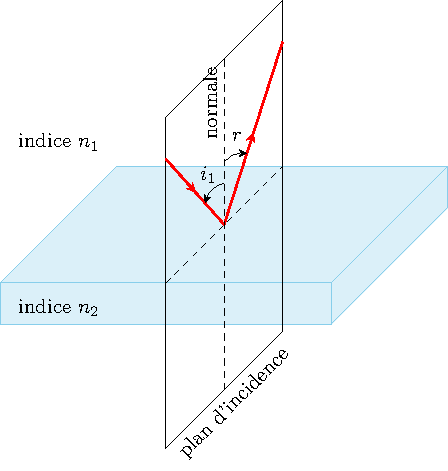
\includegraphics[width=\linewidth]{snell_refl}
			\captionof{figure}{Réflexion d'un rayon incident}
			\label{fig:snell_refl}
		\end{center}
	\end{minipage}
	\hfill
	\begin{minipage}{0.45\linewidth}
		\begin{center}
			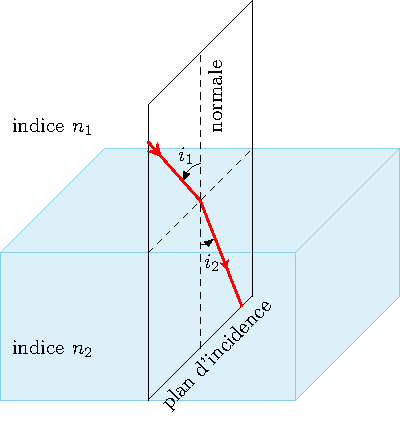
\includegraphics[width=\linewidth]{snell_refr_nsup}
			\captionof{figure}{Réfraction d'un rayon incident avec $n_2 > n_1$.}
			\label{fig:snell_refl}
		\end{center}
	\end{minipage}
\end{tcb*}

\begin{tcb*}[label=impl:refr](impl){Réfraction}
	On distingue 3 cas généraux pour la réfraction~:
	\begin{enumerate}
		\item Si $\mathbf{i_1 = 0}$,
		      \psw{%
			      alors $i_2 = 0$~: en incidence dite
			      «~normale~», il n'y a \textbf{pas de déviation} du rayon~;
		      }%
		\item Si $\mathbf{n_2 > n_1}$\footnote{On dit alors que le milieu 2 est
			      \textit{plus réfringent} que le milieu 1.},
		      \psw{%
			      alors $ \left| i_2 \right| < \abs{i_1} $~: le rayon réfracté se
			      \textbf{rapproche} de la normale~;
		      }%
		\item Si $\mathbf{n_2 < n_1}$\footnote{On dit alors que le milieu 2 est
			      \textit{moins réfringent} que le milieu 1.},
		      \psw{%
			      alors $|i_2| > |i_1|$~: le rayon réfracté \textbf{s'écarte} de la
			      normale.
		      }%
	\end{enumerate}
	Par le principe du \textit{retour inverse de la lumière}, le troisième point
	se déduit du deuxième.
\end{tcb*}

\subsection{Phénomène de réflexion totale}

À partir du moment où $n_2 > n_1$, le rayon réfracté se rapproche toujours de la
normale, et existera toujours. En revanche, si $n_1 > n_2$, le rayon réfracté
s'écarte de la normale. On considère qu'il existe uniquement s'il reste à
l'intérieur du milieu $n_2$, soit par définition $|i_2| <
	\frac{\pi}{2}\si{rad}$.

\begin{tcb*}[label=prop:ilim](prop){Angle limite de réflexion totale}
	Lors du passage d'un milieu plus réfringent à un milieu moins réfringent
	($n_1 > n_2$), il existe un angle incident limite $i_{\lim}$ au-delà
	duquel il n'y a pas de rayon réfracté~: on parle de \textbf{réflexion
		totale}. On a
	\psw{%
	\[
		\boxed{|i_{\lim}| = \arcsin \left( \frac{n_2}{n_1} \right)}
	\]
	}%
\end{tcb*}
\begin{tcb*}[label=demo:ilim](demo){Angle limite de
			réflexion totale}
	\psw{%
		Soit $i_{\rm lim}$ l'angle d'incidence limite de réfraction, tel que
		$i_2 = \frac{\pi}{2}$. On a~:
		\begin{equation*}
			i_2 = \frac{\pi}{2} \Rightarrow \sin(i_2) = 1
		\end{equation*}
		Or, $n_2\sin(i_2) = n_1\sin(i_{\rm lim})$ d'après la loi de
		Snell-Descartes pour la réfraction. Ainsi,
		\begin{align*}
			n_2 \underbrace{\cancel{\sin(i_2)}}_{=1} & = n_1\sin(i_{\rm lim})                   \\
			\Leftrightarrow \frac{n_2}{n_1}          & = \sin(i_{\rm lim})                      \\
			\Rightarrow i_{\rm lim}                  & = \arcsin \left( \frac{n_2}{n_1} \right)
		\end{align*}
	}%
\end{tcb*}
\begin{tcb}[label=exem:ilim](exem)<lftt>{Réflexion totale}
	\begin{center}
		\sswitch{
			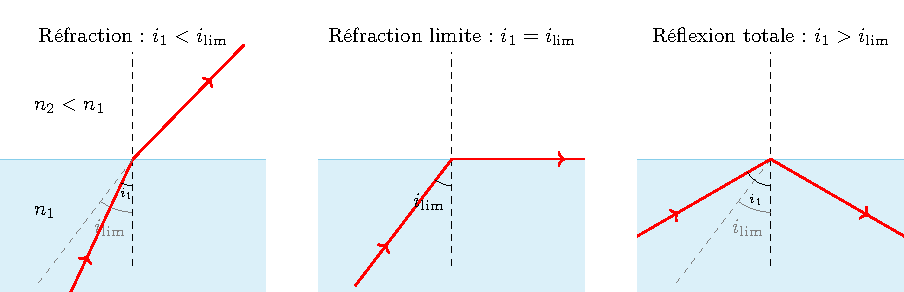
\includegraphics[width=\linewidth, draft=true]{snell_refl_tot}
			\label{fig:refl_tot}
		}{
			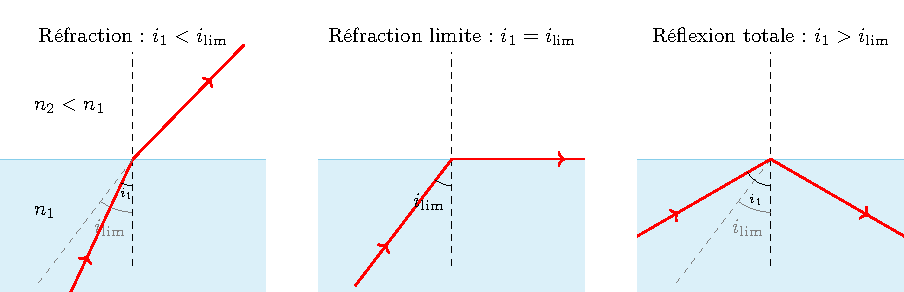
\includegraphics[width=\linewidth]{snell_refl_tot}
			\label{fig:refl_tot}
		}%
		\captionsetup{justification=centering}
		\captionof{figure}{Phénomène de réflexion totale}
	\end{center}
\end{tcb}

% \subsection{Application~: fibre optique à saut d'indice}
% Les câbles à fibres optiques permettent la transmission à haut débit de tous
% 	types de signaux électromagnétiques, sur de longues distances avec très peu
% 	d'atténuation~; ceux-ci se quesagent comme la lumière. Chaque câble comporte un
% 	grand nombre de fibres très fines.
%
% 	Une fibre optique à saut d'indice peut être assimilée à un cylindre de
% 	révolution d'axe O$z$, constitué d'un cœur de rayon $a$ (de l'ordre de 8 à
% 	\SI{50}{\micro m}) et d'indice $n_1$, entouré d'une couche cylindrinque appelée
% 	\textit{gaine}, d'épaisseur $b-a$ et d'indice $n_2 < n_1$.
%
% 	\begin{figure}[h]
% 		\centering
% 		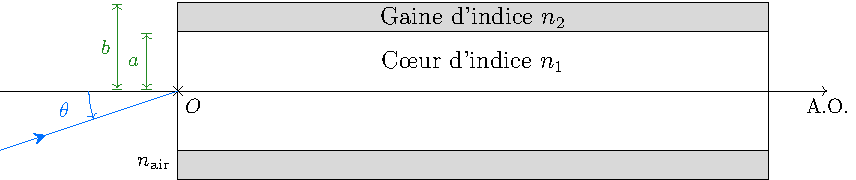
\includegraphics[width=.8\linewidth]{fibre_plain.pdf}
% 		\captionsetup{justification=centering}
% 		\caption{Schéma d'une fibre optique à saut d'indice.}
% 		\label{fig:fibre_plain}
% 	\end{figure}
%
%   \paragraph*{Principe}
% 	Un rayon pénètre depuis l'air dans la fibre par sa base en O, en faisant un
% 	angle $\theta$ avec l'axe optique confondu avec O$z$. Il subit une réfractoin
%   de l'air d'indice $n\air$ vers le cœur d'indice $n_1$. S'il arrive assez
%   rasant au niveau de l'interface cœur/gaine, comme $n_2 < n_1$ il peut subir
%   une réflexion totale, et ainsi se propager le long de la fibre sans en sortir.
%
%   \paragraph*{Angle d'acceptance}
%   Il s'agit de l'angle $\tt$ maximal tel que le rayon ne se propage que dans le
%   cœur.

\section{Généralités sur les systèmes optiques}
\subsection{Système, rayons, faisceaux.}

\begin{tcbraster}[raster columns=3, raster equal height=rows]
	\begin{tcb*}[label=def:so, raster multicolumn=2](defi){Système optique}
		\psw{%
			On appelle \textbf{système optique} un \xul{ensemble de composants} optiques
			(dioptres, miroirs) rencontrés successivement par les rayons lumineux.
		}%
	\end{tcb*}
	\begin{tcn}(exem)<rgtt>'r'{Exemple}
		L'exemple le plus simple est le miroir plan.
	\end{tcn}
\end{tcbraster}

\begin{tcb*}[label=def:vocso, sidebyside, righthand ratio=.4](defi){Système
			centré, axe optique}
	\psw{%
		C'est un système \textbf{invariant par rotation} autour d'un axe.
		\bigbreak
		On l'appelle \textit{axe optique}. \textbf{On l'oriente dans le sens de
			propagation de la lumière incidente}.
	}%
	\tcblower
	\begin{center}
		\sswitch{
			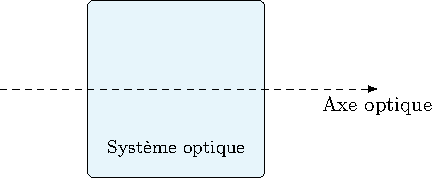
\includegraphics[width=\linewidth, draft=true]{syst_opt}
			\label{fig:socent}
		}{
			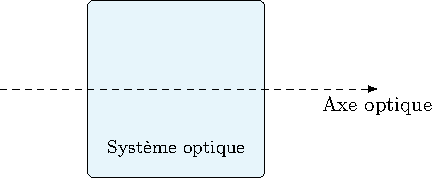
\includegraphics[width=\linewidth]{syst_opt}
			\label{fig:socent}
		}%
		\captionof{figure}{Système optique centré.}
	\end{center}
\end{tcb*}
Les distances sont considérées \textbf{algébriquement} (affectées d'un signe)~:
c'est une distance qui s'exprime en mètres, mais peut être négative selon
l'orientation de l'axe optique et de la position relative des points.
\begin{figure}[htbp]
	\centering
	\sswitch{
		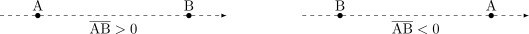
\includegraphics[scale=1, draft=true]{dist_alg}
	}{
		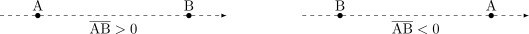
\includegraphics[scale=1]{dist_alg}
	}%
	\caption{Distances algébriques.}
	\label{fig:dist_alg}
\end{figure}

\begin{tcb*}[label=def:rlie, sidebyside, righthand ratio=.4](defi){Rayons
			incidents et émergents}
	\begin{itemize}[label=$\diamond$, leftmargin=10pt]
		\item[b]{Rayons incidents}~: \psw{entrent par la face d'entrée.}
		\item[b]{Rayons émergents}~: \psw{sortent par la face de sortie.}
	\end{itemize}
	\tcblower
	\begin{center}
		\sswitch{
			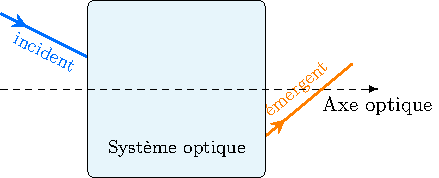
\includegraphics[width=\linewidth, draft=true]{syst_opt_ie}
			\label{fig:socent}
		}{
			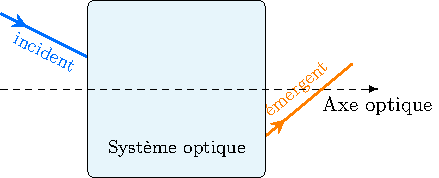
\includegraphics[width=\linewidth]{syst_opt_ie}
			\label{fig:socent}
		}%
		\captionof{figure}{Rayons incidents, émergents.}
	\end{center}
\end{tcb*}

\begin{tcb*}[label=def:faisceau, sidebyside,
		lefthand ratio=.3](defi){Nature d'un faisceau}
	\begin{itemize}[label=$\diamond$, leftmargin=10pt]
		\item[b]{Convergent}~: \psw{intersection \textbf{dans le sens direct de
				propagation}.}
		\item[b]{Divergent}~: \psw{intersection \textbf{dans le sens inverse de
				propagation}.}
		\item[b]{Parallèle}~: \psw{pas d'intersection.}
	\end{itemize}
	\tcblower
	\begin{center}
		\sswitch{
			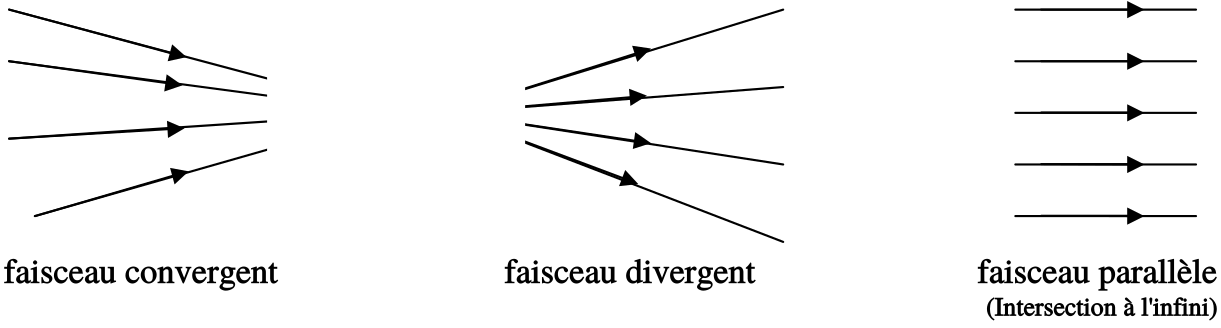
\includegraphics[width=\linewidth, draft=true]{ch2_fig8.png}
			\label{fig:faisceau}
		}{
			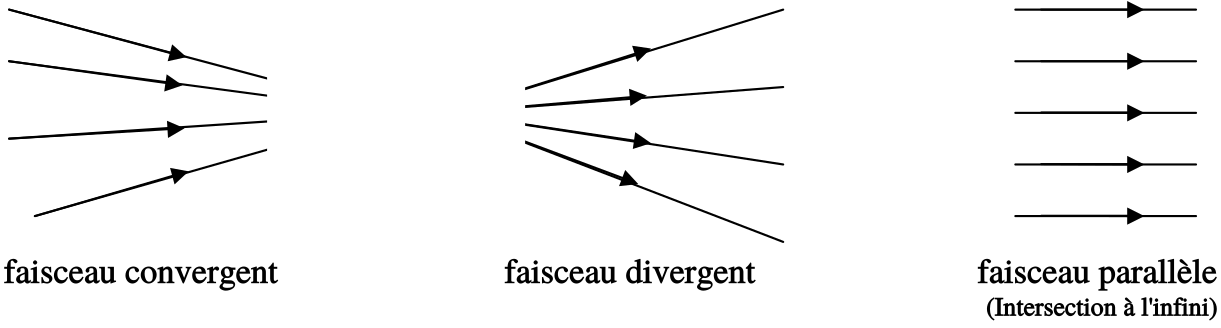
\includegraphics[width=\linewidth]{ch2_fig8.png}
			\label{fig:faisceau}
		}%
		\captionof{figure}{Natures de faisceaux}
	\end{center}
\end{tcb*}

\subsection{Objets et images}

\begin{tcb*}[label=def:objimg, sidebyside](defi){Objet et image}
	\tcbsubtitle{\fatbox{Point objet}}
	\psw{Point d'intersection des rayons \textbf{incidents}.}
	\tcblower
	\tcbsubtitle{\fatbox{Point image}}
	\psw{Point d'intersection des rayons \textbf{émergents}.}
\end{tcb*}

\begin{tcb*}[label=reelvirt, sidebyside](defi){Réel et virtuel}
	Un point \textbf{objet} est \textbf{réel} s'il est placé \textbf{avant la
		face d'entrée} du système, et \textbf{virtuel sinon}.
	\tcblower
	Un point \textbf{image} est \textbf{réel} s'il est placé \textbf{après la
		face de sortie} du système, et \textbf{virtuel sinon}.
\end{tcb*}

On trouve aussi les définitions suivantes, plus communément admises (mais plus
verbeuses).

\begin{tcb*}[label=reelvirt2, sidebyside](defi){{Réel et virtuel, bis}}
	\tcbsubtitle{\fatbox{Point objet}}
	\begin{itemize}[label=$\diamond$, leftmargin=10pt]
		\item[b]{Réel}: \psw{faisceau incident \textbf{divergent}.}
		\item[b]{Virtuel}: \psw{faisceau incident \textbf{convergent}.}
	\end{itemize}
	\tcblower
	\tcbsubtitle{\fatbox{Point image}}
	\begin{itemize}[label=$\diamond$, leftmargin=10pt]
		\item[b]{Réel}: \psw{faisceau émergent \textbf{convergent}.}
		\item[b]{Virtuel}: \psw{faisceau émergent \textbf{divergent}.}
	\end{itemize}
\end{tcb*}

\begin{tcb}[label=exem:rellvirt](exem)<lftt>{Objets et images réelles ou virtuelles}
	\begin{minipage}{0.45\linewidth}
		\begin{center}
			\sswitch{%
				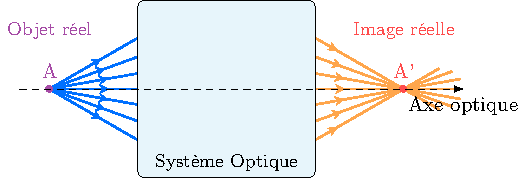
\includegraphics[width=\linewidth, draft=true]{obj_r-img_r}
			}{%
				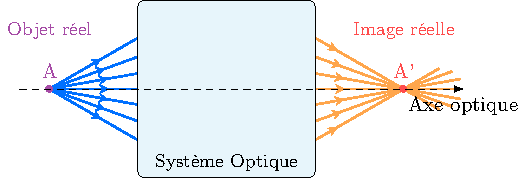
\includegraphics[width=\linewidth]{obj_r-img_r}
			}%
			\vspace{-15pt}
			\captionof{figure}{Objet et image réelles.}
			\label{fig:objrimgr}
		\end{center}
	\end{minipage}
	\hfill
	\begin{minipage}{0.45\linewidth}
		\begin{center}
			\sswitch{%
				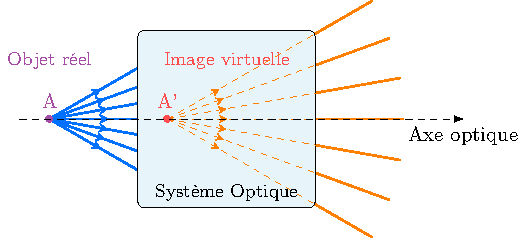
\includegraphics[width=\linewidth, draft=true]{obj_r-img_v}
			}{%
				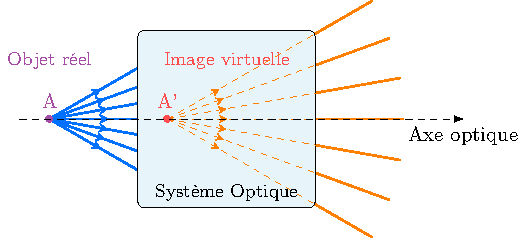
\includegraphics[width=\linewidth]{obj_r-img_v}
			}%
			\vspace{-15pt}
			\captionof{figure}{Objet réel et image virtuelle.}
			\label{fig:objrimgv}
		\end{center}
	\end{minipage}
	\begin{minipage}{0.45\linewidth}
		\begin{center}
			\sswitch{%
				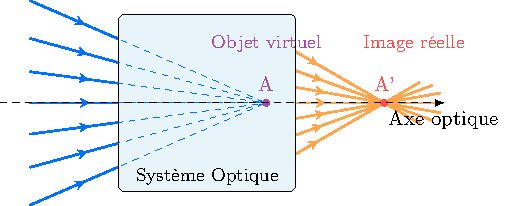
\includegraphics[width=\linewidth, draft=true]{obj_v-img_r}
			}{%
				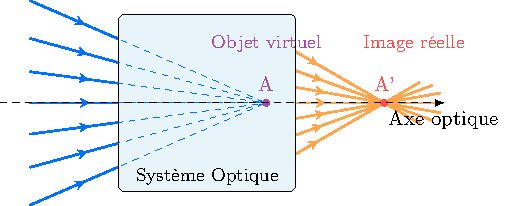
\includegraphics[width=\linewidth]{obj_v-img_r}
			}%
			\vspace{-15pt}
			\captionof{figure}{Objet virtuel et image réelle.}
			\label{fig:objvimgr}
		\end{center}
	\end{minipage}
	\hfill
	\begin{minipage}{0.45\linewidth}
		\begin{center}
			\sswitch{%
				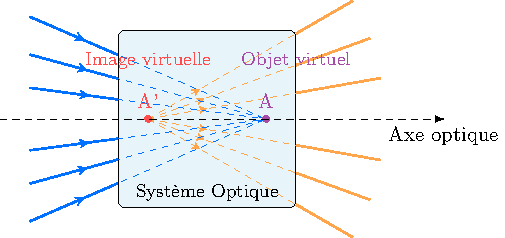
\includegraphics[width=\linewidth, draft=true]{obj_v-img_v}
			}{%
				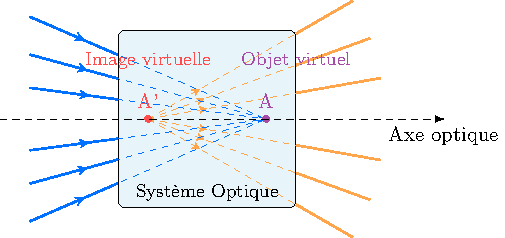
\includegraphics[width=\linewidth]{obj_v-img_v}
			}%
			\vspace{-15pt}
			\captionof{figure}{Objet et image virtuelles.}
			\label{fig:objvimgv}
		\end{center}
	\end{minipage}
	\vspace{-10pt}
\end{tcb}

\begin{tcb*}[label=impl:objimg_espace](impl){Espaces objet et image}
	Zones spatiales d'un système optique où un objet ou une image sera réel-le ou
	virtuel-le.
	\begin{center}
		\sswitch{
			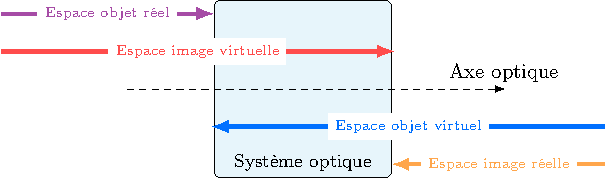
\includegraphics[width=.5\linewidth, draft=true]{objimg_espace}
			\label{fig:objimg_espace}
		}{
			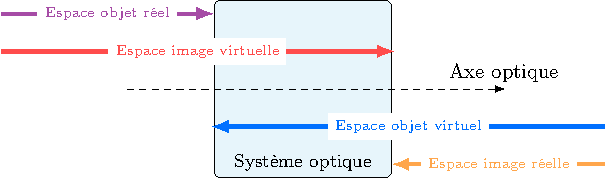
\includegraphics[width=.5\linewidth]{objimg_espace}
			\label{fig:objimg_espace}
		}%
		\captionof{figure}{Espaces objet et image.}
	\end{center}
\end{tcb*}

\begin{tcb*}[label=def:conjug](defi){Conjugaison de 2 points}
	Un objet A et son image A' par un système S sont dits \textbf{conjugés}.
	On note~:
	\psw{%
		\[
			\boxed{\rm A\opto{S}{}A'}
		\]
	}%
	avec A un objet \textbf{pour S}, et A' est une image \textbf{pour S}.
\end{tcb*}

\begin{tcb*}[label=def:objet](defi){Objet étendu et angle apparent}
	\begin{itemize}[label=$\diamond$, leftmargin=10pt]
		\item[b]{Objet étendu}~: \psw{%
			ensemble de points objets continu,
			considéré comme une infinité de points objets
		}%
		\item[b]{Angle apparent} d'un objet étendu~: \psw{%
			angle perçu (par un
			détecteur~: œil, caméra…) entre les rayons émis par les extrémités de
			l'objet.
		}%
	\end{itemize}
\end{tcb*}
\begin{tcb*}[label=def:grand, sidebyside](defi){Grandissement transversal}

	Soit $\AB$ un objet étendu avec A sur l'axe optique, passant par
	un système S donnant une image elle aussi étendue $\ABp$. On
	appelle \textit{grandissement transversal} et on le note $\gamma$ le
	rapport
	\psw{%
		\[
			\boxed{\gamma = \frac{\ABp}{\AB}}
		\]
	}%
	pour $\ABr \opto{\rm  S}{} \ABpr$
	\tcblower
	\begin{center}
		\sswitch{
			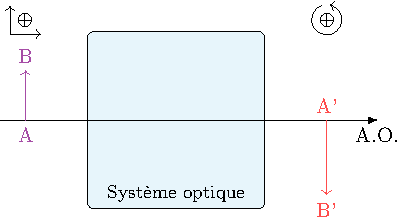
\includegraphics[width=\linewidth, draft=true]{syst_opt_objet}
			\label{fig:obj_et}
		}{
			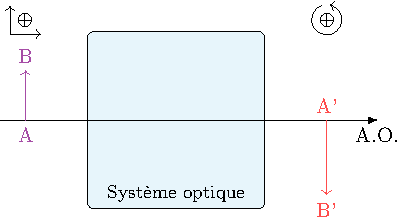
\includegraphics[width=\linewidth]{syst_opt_objet}
			\label{fig:obj_et}
		}%
		\vspace{-15pt}
		\captionof{figure}{Objet et image étendues.}
	\end{center}
\end{tcb*}

\vspace{-15pt}
\subsection{Foyers d'un système optique}

\begin{tcb*}[label=def:foy, sidebyside, sidebyside align=top](defi){Foyers
			principaux image et objet}
	\tcbsubtitle{\fatbox{Foyer principal objet}}
	Noté $F$, c'est le \textbf{point objet} dont \textbf{l'image est à l'infini}
	avec des rayons parallèles à l'axe optique.
	\smallbreak
	Le plan perpendiculaire à l'axe optique et passant par $F$ est appelé
	\textit{plan focal objet}, $\pi$. On note
	\smallbreak
	\psw{%
		\[
			\boxed{{\rm F} \opto{S}{} \underset{\text{sur l'axe optique}}{\infty}}
		\]
	}%
	\begin{center}
		\sswitch{ 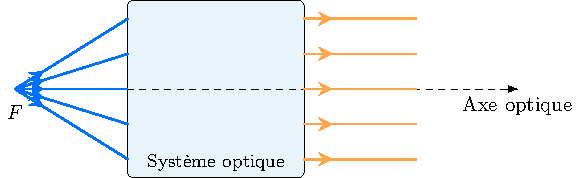
\includegraphics[height=2.5cm, draft=true]{fobj}
			\label{fig:fobj}
		}{
			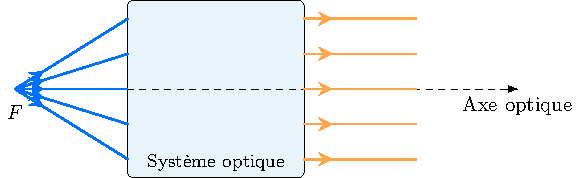
\includegraphics[height=2.5cm]{fobj}
			\label{fig:fobj}
		}%
		\captionof{figure}{Foyer principal objet.}
	\end{center}
	\tcblower
	\tcbsubtitle{\fatbox{Foyer principal image}}
	Noté $F'$, c'est le \textbf{point image} dont \textbf{l'objet est à l'infini}
	avec des rayons parallèles à l'axe optique.
	\smallbreak
	Le plan perpendiculaire à l'axe optique
	et passant par $F'$ est appelé \textit{plan focal image}, $\pi'$. On note
	\smallbreak
	\psw{%
		\[
			\boxed{\underset{\text{sur l'axe optique}}{-\infty} \opto{S}{} {\rm F'}}
		\]
	}%
	\begin{center}
		\sswitch{
			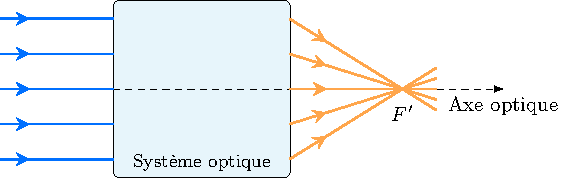
\includegraphics[height=2.5cm, draft=true]{fimg}
			\label{fig:fimg}
		}{
			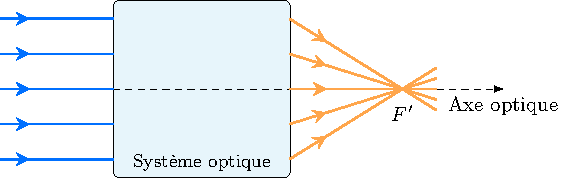
\includegraphics[height=2.5cm]{fimg}
			\label{fig:fimg}
		}%
		\captionof{figure}{Foyer principal image.}
	\end{center}
\end{tcb*}

\begin{tcb}[label=rema:retinv](rema)<lftt>{Retour inverse}
	Nous pouvons en quelque sorte déduire le fonctionnement du système
	optique dans le second cas en utilisant le principe du \textbf{retour
		inverse de la lumière}, en «~remontant le film~».
\end{tcb}
\begin{tcbraster}[raster multicolumn=2]
	\begin{tcb*}[label=prop:foy](prop){Foyers principaux}
		\begin{itemize}[label=$\diamond$, leftmargin=10pt]
			\item Rayons \textbf{incidents croisés en F} $\Ra$ \psw{%
				      \textbf{émergent parallèles} à l'axe optique~;
			      }%
			\item Rayons \textbf{incidents parallèles à l'axe} $\Ra$ \psw{%
				      \textbf{émergent croisés en F'}.
			      }%
		\end{itemize}
	\end{tcb*}
	\begin{tcb*}[label=coro:foysec](coro)'r'{Foyers secondaires}
		\begin{itemize}[label=$\diamond$, leftmargin=10pt]
			\item Rayons \textbf{incidents $\parr$ entre eux} $\Ra$ \psw{%
				      émergent \textbf{croisés en $\f' \in \pi'$}~;
			      }%
			\item Rayons \textbf{incidents croisés en $\f \in \pi$} $\Ra$ \psw{%
				      émergent \textbf{parallèles entre eux}.
			      }%
		\end{itemize}
	\end{tcb*}
\end{tcbraster}

\section{Approximation de \textsc{Gauss}}

\subsection{Stigmatisme, aplanétisme}

\begin{tcbraster}[raster columns=2, raster equal height=rows]
	\begin{tcb*}[label=def:stig](defi){Stigmatisme}
		\psw{%
			\textbf{Stigmatique} $\Lra$ rayons émis par un point objet $A$ convergent
			en \textbf{un seul point} image $A'$. Inverse~: l'image d'un point forme
			une \textbf{tâche}.
		}%
	\end{tcb*}
	\begin{tcb*}[label=def:apla](defi)'r'{Aplanétisme}
		\psw{%
			\textbf{Aplanétique} $\Lra$ objet étendu $\AB$ $\perp$ à l'axe
			$\Ra$ une image $\ABp$ également $\perp$ à l'axe.
		}%
	\end{tcb*}
\end{tcbraster}

\subsection{Rigoureux ou approché~?}

La plupart des systèmes optiques (lentilles, œil, appareil photo…) ne sont pas
rigoureusement stigmatiques et aplanétiques~: il arrive souvent qu'un point
source forme une tâche sur un capteur (astigmatisme) ou qu'une droite soit vue
courbée (non-aplanétisme). On peut cependant trouver des conditions
dans lesquelles le stigmatisme et l'aplanétisme sont approchés, par exemple si
la tâche formée par le système est plus petite que l'élément récepteur (pixel
pour une caméra).

\begin{figure}[htbp]
	\centering
	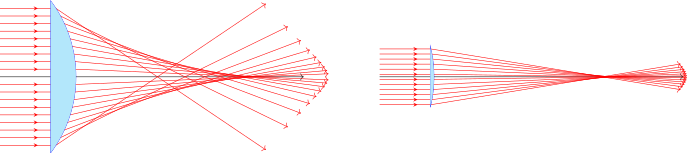
\includegraphics[scale=.95]{stig}
	\caption{Exemple d'un système astigmatique à gauche, stigmatique approché à
		droite.}
	\label{fig:stig}
\end{figure}

\vspace{-15pt}
\subsection{Conditions de \textsc{Gauss}}

\begin{tcb*}[label=def:gausscond](defi){Rayons paraxiaux}
	Des rayons sont \textbf{paraxiaux} s'ils sont~:
	\begin{enumerate}
		\item \psw{peu éloignés de l'axe optique~;}
		\item \psw{peu inclinés par rapport à l'axe optique.}
	\end{enumerate}
\end{tcb*}
\begin{tcb*}[label=prop:gaussprop](prop)'r'{Approximation de \textsc{Gauss}}
	Un système est dans les les conditions de \textsc{Gauss} si les rayons sont
	paraxiaux. Dans ce cas, un système centré respecte les conditions de
	\textbf{stigmatisme et d'aplanétisme} \textit{approchés}. On
	les \textbf{considérera} comme rigoureux tant dans les tracés que dans les
	calculs.
\end{tcb*}
\vspace{-15pt}
\end{document}
